\section{OpenHAB}
"'\textbf{OpenHAB}"'\footnote{\textbf{open} \textbf{H}ome \textbf{A}utomation \textbf{B}us} ist eine Software, die Komponenten für die Hausautomation verschiedenster Hersteller auf einer Plattform vereint. Als UI werden Webbrowser, Android- oder iOS-Systeme unterstützt. Die aktuelle Version ist OpenHAB 2 (Stand: 19.07.2017). \newline

\subsection{Installation auf Linux (Raspbian Jessie)}

\begin{enumerate}
	\item Schlüssel für Bintray Paketquelle hinzufügen \newline
	\texttt{wget -qO - 'https://bintray.com/user/downloadSubjectPublicKey?username=\\openhab' | sudo apt-key add -}
	
	\item Apt erlauben, das HTTPS-Protokoll zu nutzen\newline
	\texttt{sudo apt-get install apt-transport-https}
	
	\item OpenHAB 2 Paketquelle (stabile Version) in die Quellenliste kopieren\newline
	\texttt{echo 'deb https://dl.bintray.com/openhab/apt-repo2 stable main' | sudo tee /etc/apt/sources.list.d/openhab2.list}
	
	\item Paketindex erneuern\newline
	\texttt{sudo apt-get update}
	
	\item OpenHAB 2 installieren\newline
	\texttt{sudo apt-get install openhab2}
	
	\item \textbf{Optional}: Um die Komponenten für die Hausautomatisierung zu steuern, werden bei OpenHAB Add-Ons bzw. Bindings installiert. Diese werden üblicherweise aus dem Internet heruntergeladen. Möchte man jedoch auch offline Add-Ons installieren können, besteht die Möglichkeit, das Add-Ons-Package zu installieren, sodass man auch ohne Internet zusätzliche Module installieren kann. Dies geschieht mit : \texttt{sudo apt-get install openhab2-addons} \cite{c2}
	
	\item OpenHAB 2 starten (das erste Starten kann bis zu 15 Minuten dauern)
	
	\texttt{sudo systemctl start openhab2.service}\newline
	\texttt{sudo systemctl daemon-reload}\newline
	\texttt{sudo systemctl enable openhab2.service}\newline
	
	Abfragen des Status:\newline
	\texttt{sudo systemctl status openhab2.service}
	
\end{enumerate}

\newpage

\textbf{Konfiguration}

Nach der Installation sollte unter \texttt{https://localhost:8080} (\texttt{https://ipadressedes-\\openhabservers:8080}) das OpenHAB2-Portal (s. Abb. \ref{fig:ohportal}) erreichbar sein.

\begin{figure}[H]
	\centering
	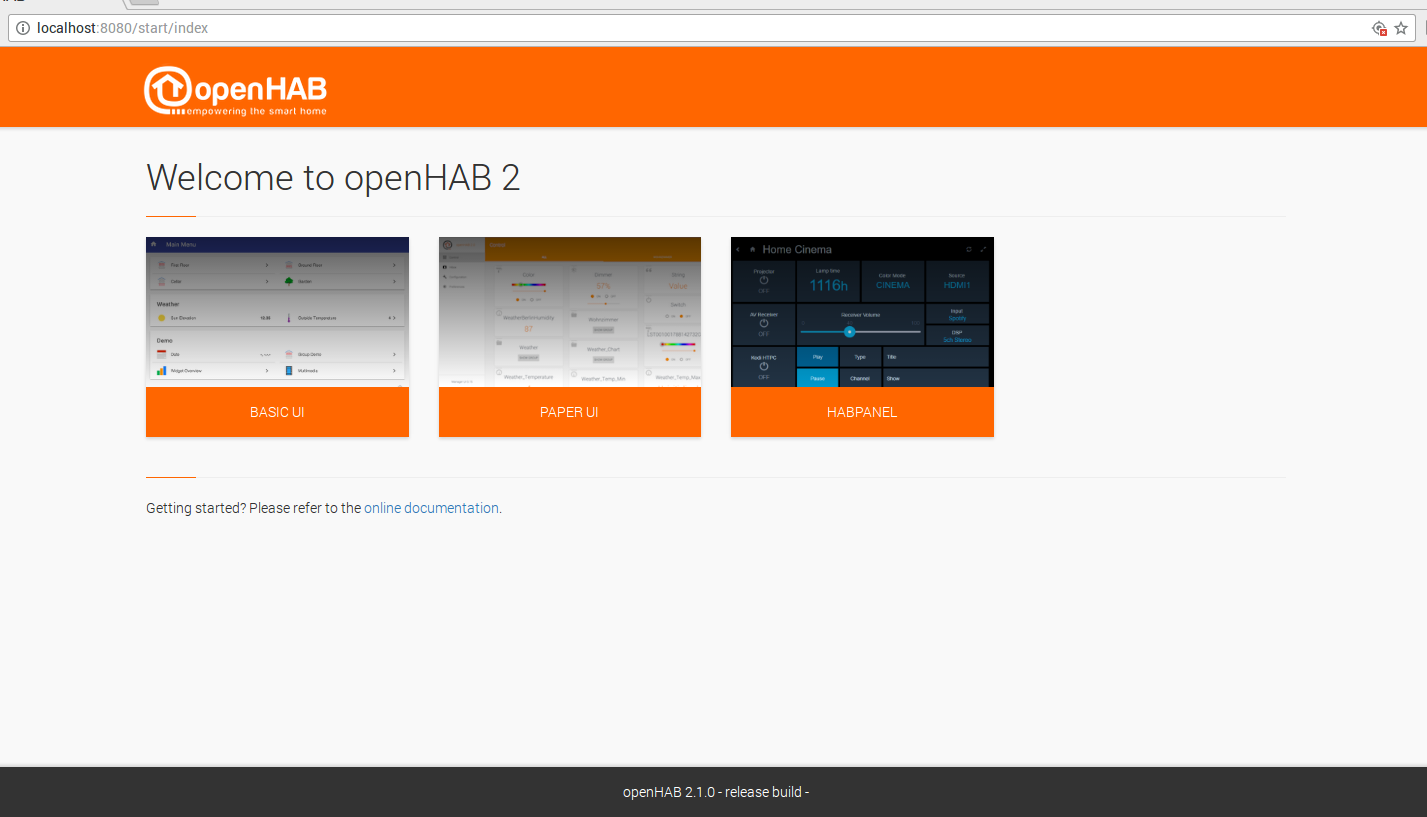
\includegraphics[width=1\textwidth]{Bilder/ohPortal}
	\caption{OpenHAB2-Portal}
	\label{fig:ohportal}
\end{figure}

Dort kann man zwischen drei verschiedenen Oberflächen wählen. Das "'\textbf{Basic UI}"' und "'\textbf{HAB Panel}"' werden dabei rein für die Darstellung und Steuerung der verschiedenen Komponenten des Smarthomes genutzt.

Zur Konfiguration von OpenHAB wird das "'\textbf{Paper UI}"' genutzt.
Dort können unter der Option "'\textbf{Add-Ons}"' unter "'\textbf{Bindings}"' neue Module installiert werden. Sie stellen die Schnittstelle zwischen dem Programm und der Hardware bzw. den Smart-Home-Komponenten dar.\newline


\subsection{Items}
Items sind die Grund-Datentypen in OpenHAB. Mit ihnen lassen sich die Komponenten des Smarthomes steuern. So kann man mit einem Item des Typs "'Switch"' schaltbare Steckdosen, Relais, etc. schalten. Alle möglichen Typen sind in \autoref{tbl:items} aufgeführt.

\begin{table}[H]
	\centering
	\setlength\extrarowheight{2pt}
	\begin{tabularx}{\textwidth}{LXX}  
		\toprule
		\textbf{Typ} & \textbf{Beschreibung} & \textbf{Mögliche Befehle}\\
		\midrule
		Color 	&  Speichert Farbinformation (RGB) &   OnOff, IncreaseDecrease, Percent, HSB 	\\
		Contact	&  Speichert Status von elektrischen Kontakten. Enthält nur Statusinformation, keine Befehle möglich. &	OpenClosed    \\
		DateTime   &	Speichert Datum und Uhrzeit & - \\
		Dimmer   & Wert für Dimmern (in Prozent) & OnOff, IncreaseDecrease, Percent\\
		Group   & Gruppiert mehrere Items zu einem Item. & -\\
		Image   & Binärdaten eines Bildes & -\\
		Location   & GPS Koordinaten & Point\\
		Number   & Zahlenwert & Decimal\\
		Player  & Kontrolle über Player (z.B. Audio-Player) & PlayPause, NextPrevious, RewindFastforward\\
		Rollershutter & Kontrolle über Rolladen& UpDown, StopMove, Percent\\
		String & Speichert Text & String \\
		Switch & An/Aus-Schalter& OnOff\\
		\bottomrule 
	\end{tabularx}
	\caption{Item-Datentypen und jeweils möglichen Befehlen}
	\label{tbl:items}
\end{table}

\subsection{Things}
\subsection{Sitemap}

\begin{table}[H]
	\centering
	\setlength\extrarowheight{2pt}
	\begin{tabularx}{\textwidth}{LX}  
		\toprule
		\textbf{Element} & \textbf{Beschreibung}\\
		\midrule
		Chart 	&  Diagramm\\
		Colorpicker	&  Farbauswahl \\
		Default   &	Rendert ein Objekt abhängig vom Itemtyp \\
		Frame   & Gruppierung/Umrahmung mehrerer Sitemap-Elemente. \\
		Group   & Gruppiert die angegebenen Elemente in einen Block.\\
		Image   & Bild (gegeben durch URL)\\
		Mapview   & OSM Karte \\
		Selection   & Dropdown Menü um ein Item auszuwählen \\
		Setpoint  & Wert mithilfe +/- Buttons auswählen \\
		Slider & Schieberegler \\
		Switch & An/Aus-Schalter \\
		Text & Beschriftung \\
		Video & Zeigt ein Video (angegeben durch URL) \\
		Webview & Zeigt Inhalt einer Webseite.\\
		\bottomrule 
	\end{tabularx}
	\caption{Sitemap-Typen}
	\label{tbl:sitemapss}
\end{table}



\subsection{OpenHAB Android-App}
Die OpenHAB App ist für Android und iOS verfügbar und bietet die Möglichkeit, den OpenHAB-Server bzw. OpenHAB-Cloud-Instanzen (s. \autoref{fig:ohCloud}) zu steuern.

Die App verbindet sich entweder über die lokale Server-URL (bzw. IP-Adresse) mit dem Openhab-Dashboard oder über Fernzugriff mit \texttt{https://myopenhab.org}. Hierfür muss man einen Account bei \texttt{myopenhab.org} anlegen und die Anmeldeinformationen in den Einstellungen der App eingeben.

Seitens OpenHAB muss der \textit{OpenHAB Cloud Connector} eingebunden werden und die URL für den OpenHAB Cloud Server eingegeben werden (\texttt{https://myopenhab.org}).


\paragraph{Anmerkung zur Registrierung bei myopenhab.org}

Zur Registrierung bei myopenhab.org sind unter Anderem die \textit{openHAB UUID} und das \textit{openHAB Secret} notwendig. Ersteres lässt sich mit \texttt{cat /var/lib/openhab2/uuid}, das Secret mit \texttt{cat /var/lib/openhab2/openhabcloud/secret} ausgeben.


\begin{figure}[H]
	\centering
	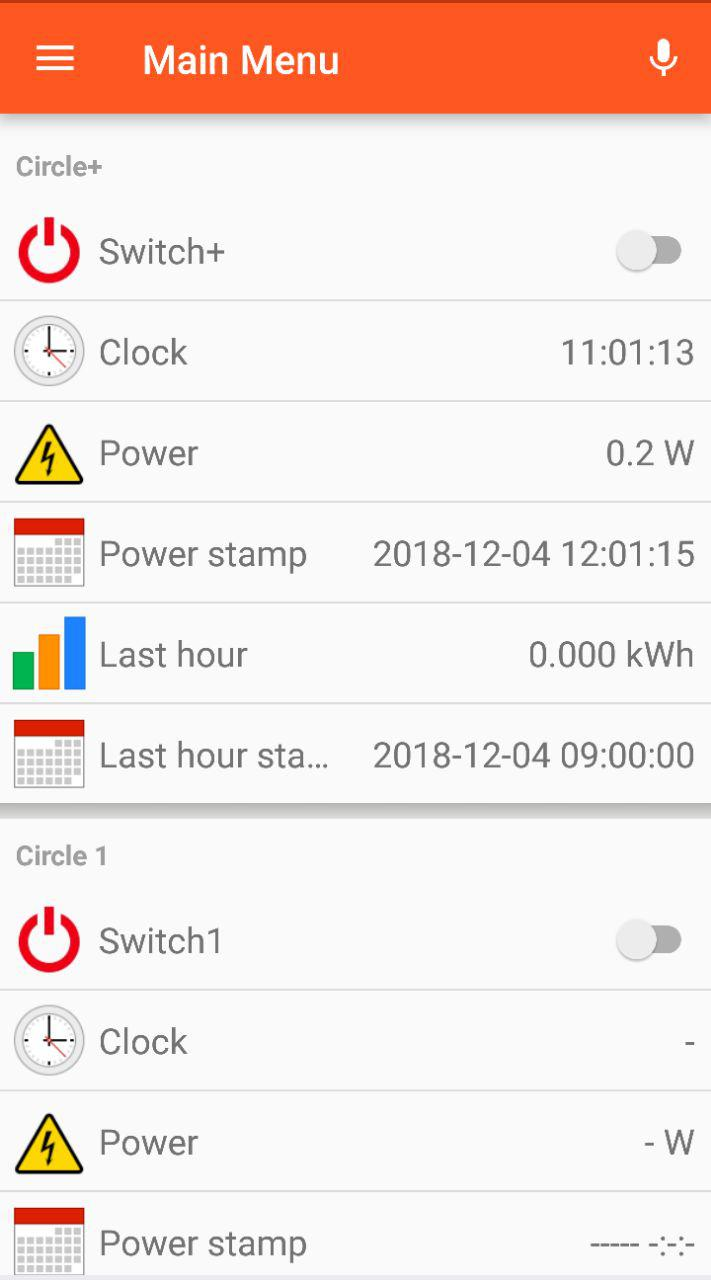
\includegraphics[width=0.3\textwidth]{Bilder/App}
	\caption{Benutzeroberfläche der OpenHAB Android App}
	\label{fig:ohCloud}
\end{figure}

\begin{figure}[H]
	\centering
	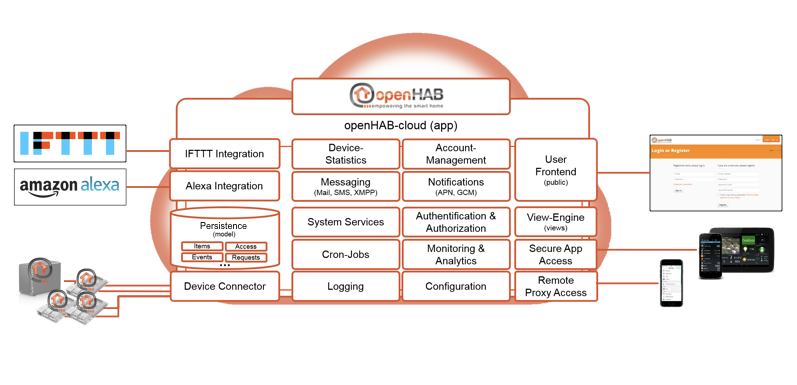
\includegraphics[width=0.9\textwidth]{Bilder/openHAB-Cloud}
	\caption{Architektur der OpenHAB-Cloud}
	\label{fig:ohApp}
\end{figure}

\newpage


\section{Schaltbare Steckdosen}
\subsection{Steckdosen von Plugwise}

Das vorhandene Set besteht aus 6 Steckdosen und einem USB-Stick zur Kommunikation mit einem Rechner. Die Steckdosen bieten neben der Möglichkeit des Ein- und Ausschaltens auch die Aufzeichnung des Stromverbrauches eines angeschlossenen Gerätes. 

\begin{figure}[h!]
	\centering
	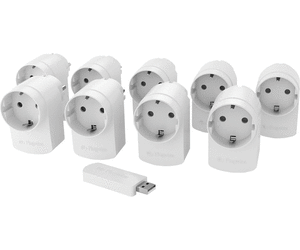
\includegraphics[width=6cm]{Bilder/pwsteckdosen.png}
	\caption{Plugwise Steckdosen mit Stick}
\end{figure}

\subsubsection{Kommunikation und Netzwerkaufbau} 

Die Steckdosen, auch "'\textbf{Circles}"' oder Module genannt, kommunizieren untereinander über das \textbf{ZigBee}-Protokoll\footnote{'ZigBee ist eine Spezifikation für drahtlose Netzwerke mit geringem Datenaufkommen, wie beispielsweise Hausautomation, Sensornetzwerke, Lichttechnik' \cite{c1}} %fußnote einfügen. \\
Die einzelnen Module werden zu einem Netzwerk zusammengefügt. Dies geschieht üblicherweise mittels der herstellereigenen Software "'\textbf{Plugwise Source}"' (nur für Windows verfügbar). Die Konfiguration des Netzwerks geschieht über das "'\textbf{Circle+}"' und den "'\textbf{Plugwise-Stick}"'. Letzterer dient als Schnittstelle zwischen Computer und Steckdosen. Das \textbf{Circle+} speichert alle dem jeweiligen Netzwerk angehörigen \textbf{Circles}, ansonsten fungiert es als gewöhnliche Funksteckdose. \newline
Die Übertragung der Daten (Status,Stromverbrauch,...) findet über Wege von Modul zu Modul statt,sodass auch weiter entfernte Geräte angesprochen werden können.\\
Zugriff auf die Module anderer Netzwerke ist mit Hilfe von zusätzlicher Hardware \\ (\textbf{Plugwise Stretch Lite}) möglich. \newline
Ein Netzwerk sollte immer so aufgebaut sein, dass \textbf{Plugwise-Stick} und \textbf{Circle+} direkten "'Sichtkontakt"' haben und jede Steckdose immer jeweils eine anderes Modul hat, an das sie Daten weiterschicken kann. Im Optimalfall (optimale Datengeschwindigkeit) ist das Netzwerk wie in Abb. \ref{fig:netzwerk} rechts angeordnet, wobei sich der \textbf{Plugwise-Stick} zudem möglichst zentral befindet.
% bild plugwise-netzwerk einfügen

%TODO Abbildung schöner zeichnen
\begin{figure}[H]
	\centering
	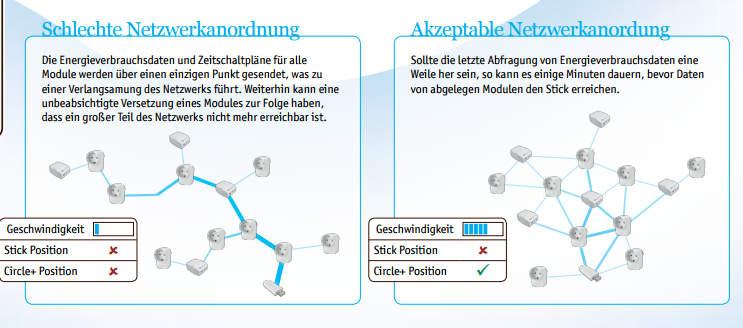
\includegraphics[width=1\textwidth]{Bilder/plugwise-netzwerk}
	\caption{Plugwise-Netzwerk}
	\label{fig:netzwerk}
\end{figure} \mbox{}

\subsubsection{Möglichkeiten zum Ansprechen der Plugwise-Steckdosen mit dem Raspberry Pi} 

\paragraph{python-plugwise (Linux)}

Das "'\textbf{python-plugwise}"' bietet unter anderem folgende Möglichkeiten:

\begin{itemize}
	\item Steckdosen einzeln ein- und ausschalten
	\item Energieverbrauch der einzelnen Steckdosen auslesen
	\item Information über die einzelnen Steckdosen auslesen
	\item Uhrzeit einstellen bzw. mit der Systemzeit synchronisieren
\end{itemize}

\subparagraph{Installation}
\begin{enumerate}
	\item Dateien unter \texttt{https://github.com/aequitas/python-plugwise} herunterladen.
	\item In der Kommandozeile zum Verzeichnis wechseln, in denen sich die Dateien befinden und "'\texttt{sudo python setup.py install}"' ausführen.
	\item Mit \texttt{plugwise\_util -h} werden alle Befehle aufgelistet.
	
\end{enumerate}

\newpage

\paragraph{OpenHAB}

Um mit OpenHAB die Plugwise-Steckdosen anzusprechen, wird zum Einen das "'\textbf{Serial-Binding}"' benötigt. Dieses erlaubt OpenHAB, mit Geräten in ASCII über die serielle Schnittstelle zu kommunizieren. Zum Anderen wird auch das "'\textbf{Plugwise-Binding}"' benötigt, durch das die Kommunikation mit den Steckdosen ermöglicht wird.\newline

\textbf{Hinweis: }

Da OpenHAB die serielle Schnittstelle nicht erkennt, muss zusätzlich in der Datei \newline \texttt{/etc/default/openhab2} die Auskommentierung von 

\texttt{EXTRA\_JAVA\_OPTS="Dgnu.io.rxtx.SerialPorts=/dev/ttyUSB0:/dev/ttyS0:/dev/\\ttyS2:/dev/ttyACM0:/dev/ttyAMA0"}

aufgehoben werden.

\newpage

\paragraph{Konfiguration des Plugwise-Bindings}

Als Erstes wird der "'\textbf{Plugwise-Stick}"' konfiguriert, hierfür bestehen zwei Möglichkeiten:
\begin{enumerate}
	\item Im '\textbf{Paper UI}' kann unter '\textbf{Configuration}' $\rightarrow$  '\textbf{Bindings}' $\rightarrow$  '\textbf{Plugwise Binding}' $\rightarrow$  '\textbf{Configure}' der serielle Port eingestellt werden. Unter Linux ist dies meist \textbf{/dev/ttyUSB0}. \newline
	Mit dem '\textbf{stick.interval}' kann das Zeitintervall eingestellt werden, mit dem Nachrichten über das '\textbf{ZigBee-Netzwerk}' geschickt werden.
	\item Die Konfiguration wird direkt in der Konfigurationsdatei des Bindings,'\textbf{plugwise.cfg}', vorgenommen. Diese findet man unter \texttt{/etc/openhab2/services}. Dort können auch die verschiedenen Module des Plugwise-Netzwerkes konfiguriert werden, wie in Listing \ref{lst:ohConfig} zu sehen ist.\newline
	
	
	\lstinputlisting[label=lst:ohConfig,caption = {Konfiguration des vorhandenen Plugwise-Netzwerkes}]{lst/plugwiseConfig.txt}
	
\end{enumerate}

\textbf{Konfiguration der Plugwise-Module}
Das '\textbf{Plugwise-Binding}' stellt verschiedene Items für die einzelnen Komponenten des Netzwerks, z.B. Circle, Stealth, Sense, etc. zur Verfügung. Da aber nur Circles und Stealths\footnote{Einbaumodule zur Messung des Energieverbrauchs} zur Verfügung stehen, beschränkt sich die hier beschriebene Konfiguration auf diese beiden Typen. \newline
Für diese Komponenten sind nachfolgend die zugehörigen Items dargestellt (s. Tabelle \ref{tbl:oh}). Die vollständige Auflistung aller Items siehe \cite{c4}.

\begin{center}
	\begin{table}[H]
		\centering
		\setlength\extrarowheight{2pt}
		\begin{tabularx}{\textwidth}{lXX}  
			\toprule
			Kommando & Item-Typ  & Funktion  \\
			\midrule
			clock 	&  String      	& Die interne Zeit des Moduls wird abgefragt.\\
			lasthour 	&  Number 		& Energieverbrauch der letzten Stunde in \SI{}{\kilo\watt\hour}\\
			lasthour- stamp &	DateTime	& Zeitstempel der letzten stündlichen Energieverbrauchabfrage\\
			power   & 	Number			& Aktueller Energieverbrauch.\\
			power-stamp       & DateTime  & Zeitstempel des aktuellen Verbrauchs     \\
			realtime-clock    & DateTime  & Interne Zeit des Circle+   \\
			\bottomrule
		\end{tabularx}
		\caption{Items des Plugwise-Bindings}
		\label{tbl:oh}
	\end{table}
\end{center}

Die Syntax zur Definition der Items ist wie folgt:

\begin{itemize}
	\item Für \textbf{Items} die einen "'\textbf{An-/Aus-Befehl}"' senden können :
	
	\texttt{plugwise="[<command>:<plugwise id>:<plugwise command>:<polling \\ interval>], [<command>:<plugwise id>:<plugwise command>:<polling
		\\ interval>], ..."}. 
	
	\texttt{command} kann dabei die Werte "'ON"' oder "'OFF"' annehmen.
	Die \texttt{plugwise-id} stellt die MAC-Adresse\footnote{Die MAC-Adressen befinden sich jeweils auf der Rückseite der Steckdosen.} des jeweiligen Gerätes (bzw. den Gerätenamen, der in der Datei "'plugwise.cfg"' festgelegt wird) dar. "'\texttt{plugwise command}"' ist der Befehl, der zum jeweiligen Gerät geschickt wird, wenn "'\texttt{command}"' übergeben wird. Mit dem "'\texttt{polling interval}"' legt man das Zeitintervall in Sekunden fest, in denen der Status des Geräts abgefragt wird.
	
	
	\item Für \textbf{Items}, die einen \textbf{Wert} speichern:
	
	\texttt{plugwise="[<plugwise id>:<plugwise variable>:<polling interval>],\newline  [<plugwise  id>:<plugwise variable>:<polling interval>], ..."}. 
	
	Hierbei ist die "'\texttt{plugwise variable}"' die Gerätestatus-Variable, die abgefragt oder "'vergeben"' wird.
	
\end{itemize}

Für das vorhandene Set an Steckdosen wurden die Items unter \texttt{/etc/openhab2/items/\\plugwise.items}, wie in Listing \ref{lst:pwItems} (Ausschnitt) aufgeführt, konfiguriert. Da die Konfiguration für alle Steckdosen gleich ist, wird nur diejenige für das Circle+ angezeigt.

\lstinputlisting[label=lst:pwItems, caption = {Konfiguration der Plugwise-Items}]{lst/pwItems.txt}

\newpage

\paragraph{Darstellung und Bedienung der Module}

Für die Darstellung und Bedienung der \textbf{Items} muss unter \texttt{/etc/openhab2/sitemaps/\mbox{} smarthome.sitemap} eine "'\textbf{Sitemap}"' definiert werden. Diese beschreibt das Aussehen der Seite auf der Benutzeroberfläche. Listing \ref{lst:pwSitemap}(gekürzt) zeigt eine beispielhafte Konfiguration. Die dazugehörige Oberfläche im "'Basic UI"' ist in Abb. \ref{fig:ohbasic} dargestellt.\newline



\begin{figure}[H]
	\centering
	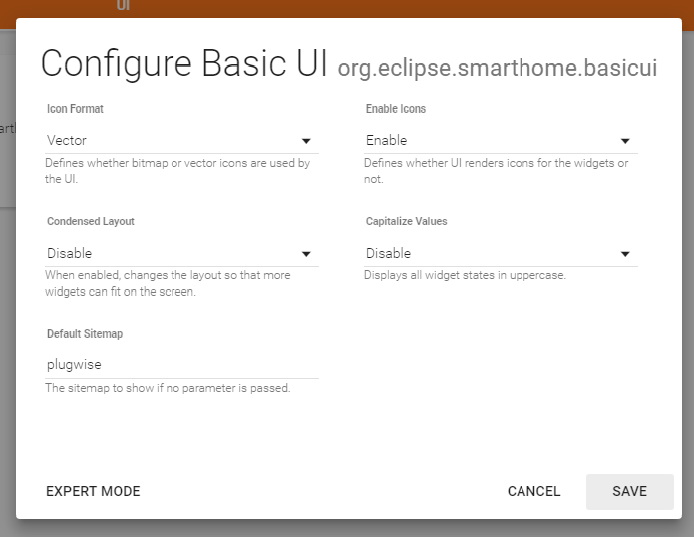
\includegraphics[width=0.5\textwidth]{Bilder/sitemapcfg}
	\caption{Sitemap-Konfiguration}
	\label{fig:sitemapcfg}
\end{figure}

\begin{figure}[H]
	\centering
	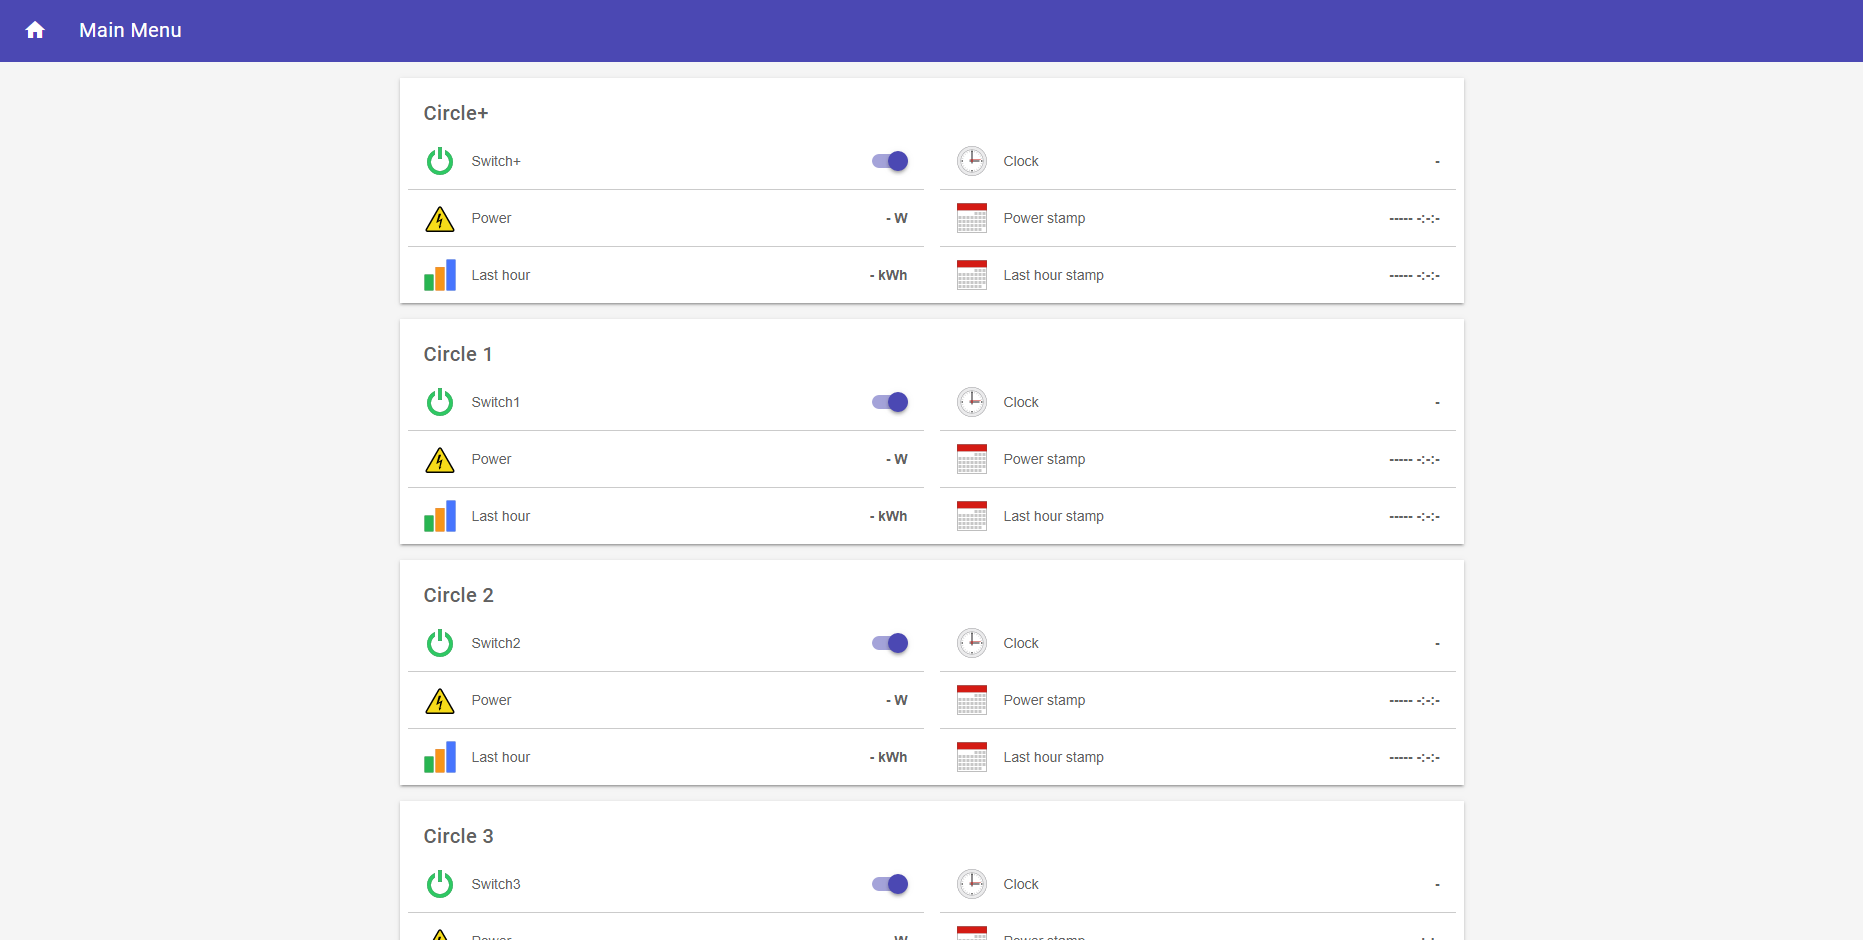
\includegraphics[width=1\textwidth]{Bilder/ohMain}
	\caption{Oberfläche im BasicUI}
	\label{fig:ohbasic}
\end{figure}

\newpage

\lstinputlisting[label=lst:pwSitemap, caption= Konfiguration der Benutzeroberfläche]{lst/pwSitemap.txt}

\textbf{Hinweis: }

Standardmäßig öffnet OpenHAB die Sitemap \textbf{default.sitemap}. Um auf die benutzerdefinierte Sitemap umzuschalten, muss deren Name (der in der ersten Zeile der Sitemap-Konfigurations-Datei definiert wird; \textbf{hier: } smarthome) im \textbf{Paper UI} unter '\textbf{Configuration}' $\rightarrow$  '\textbf{Services}' $\rightarrow$  '\textbf{Basic UI}' (oder andere Benutzeroberfläche) $\rightarrow$  '\textbf{Configure}'$\rightarrow$  '\textbf{Default Sitemap}' eingetragen werden (s. Abb. \ref{fig:sitemapcfg}). 

\newpage

\section{Präsenzerkennung}
\subsection{Bluetooth}
Zur Anwesenheitserkennung per Bluetooth kann der Ansatz gewählt werden, zunächst ein Skript zu erstellen, welches überprüft, ob ein bestimmtes Gerät vorhanden ist. Dieses Skript kann dann mit OpenHAB ausgeführt werden.

Einrichten von Bluetooth:
https://www.pi-supply.com/make/fix-raspberry-pi-3-bluetooth-issues/
\subsubsection{Vorbereitung}
\begin{itemize}
	\item \textbf{Bluetooth einrichten}
	\item \textbf{MAC-Adressen bestimmen}: Mit Hilfe \texttt{hcitool scan} lassen sich die MAC-Adressen aller Bluetooth-Geräte herausfinden, die sich gerade in der Umgebung des Pi befinden.
	\item \textbf{Bash-Skript} (hier \textbf{btSkript.sh}) zum Pingen bestimmter Bluetooth-Geräte erstellen (s. \autoref{lst:btBash}). Das Skript muss mit \texttt{chmod +x btSkript.sh} ausführbar gemacht werden. Durch \texttt{Pfad/btSkript.sh 1} bzw. \texttt{Pfad/btSkript.sh 2} kann die Funktionalität des Skripts geprüft werden. Mittels \texttt{chmod 777 btSkript.sh} wird die Ausführung der Datei für alle User, unter anderem auch OpenHAB, ermöglicht.
\end{itemize}


\lstinputlisting[label = lst:btBash, caption = Bash-Skript zur Präsenzerkennung mittels Bluetooth]{lst/bashBluetooth.txt}

\subsubsection{Einrichtung in OpenHAB}

Für die Ausführung des Skripts muss das \textbf{Exec Binding} installiert werden. Mit diesem können Kommandozeilen-Befehle ausgeführt werden. Hierfür muss ein \textbf{Thing} erstellt werden. Hierfür legt man unter \textbf{/etc/openhab2/things} eine Datei mit der Endung \textbf{.things} an, z.B. \textbf{btSkript.things}. In dieser wird jeder Befehl als Thing wie folgt definiert:
\begin{lstlisting}
Thing exec:command:bluetooth [command="sudo /home/pi/bt.sh 2", interval=10, timeout=5, autorun=false ]
\end{lstlisting}

Dadurch wird der Befehl \textbf{sudo /home/pi/bt.sh 2}, welcher überprüft, ob das Smartphone vorhanden ist, alle 10 Sekunden ausgeführt.\\
Für die Ausführung des Befehls muss jedoch noch zunächst ein \textbf{Item} erstellt werden. Hierzu wird unter \textbf{/etc/openhab/items} eine neue Datei, \textbf{anwesenheit.items}, angelegt. 
In diese trägt man die Zeile 
\begin{lstlisting}
String BT_Output "Anwesenheit [%s]" <light> {channel="exec:command:bluetooth:output"}
\end{lstlisting} ein. Dieses Item nimmt den Wert an, der durch das Ausführung des Skriptes zurückgegeben wir (also entweder "'ON"' oder "'OFF"'). "'<light>"' bezeichnet dabei das Icon, welches in der Benutzeroberfläche bei der Anwesenheit erscheint, in diesem Fall eine Glühbirne. \\


Für die Darstellung wird in der bereits beschriebenen Datei \textbf{smarthome.sitemap} der folgende Eintrag erstellt: 
\begin{lstlisting}
Text item=BT_Output label="Bluetooth [MAP(praesenz.map):%s]"
\end{lstlisting}
Außerdem muss zusätzlich das Binding \textbf{Map Transformation} (unter dem Reiter \textbf{Transformations}) installiert werden. Mit diesem können selbstdefinierte Werte, wie z.B. "'ON"' und "'OFF"', auf andere Werte bzw. Zeichenketten gemappt werden (z.B. Anwesend/Abwesend) , die dann von OpenHAB dargestellt werden. Für eine Transformation muss unter /etc/openhab2/transform eine Map-Datei (z.B. praesenz.map) erstellt werden, die folgende Form haben sollte:

\begin{lstlisting}
ON=Anwesend
OFF=Abwesend
undefined=unbekannt
\end{lstlisting}


https://klenzel.de/3328

\subsection{WLAN}
Für die Anwesenheitserkennung mit WLAN gibt es die Möglichkeit, das Network Binding zu installieren. Dieses listet alle Geräte als Things auf, die mit dem lokalen Netz verbunden sind. Nachteilig an dieser Methode ist, dass die IP-Adresse des Gerätes zur Anwesenheitserkennung genutzt wird und diese sich somit nicht ändern sollte.

\subsubsection{Einrichtung}
Sobald man das Network Binding installiert hat, kann in PaperUI unter Inbox auf verbundene Geräte überprüft werden. Hierzu klickt man auf das "'+"' und wählt im folgenden Menü Network Binding aus. Anschließend werden die IP-Adressen aller verbundenen Geräte aufgelistet. Mit einem Klick auf das Häkchen kann das gewünschte Gerät als Thing hinzugefügt werden. Nun erscheint das Gerät in Configuration unter Things. Mit einem Klick auf das Gerät erscheint folgendes Menü :
\begin{figure}[H]
	\centering
	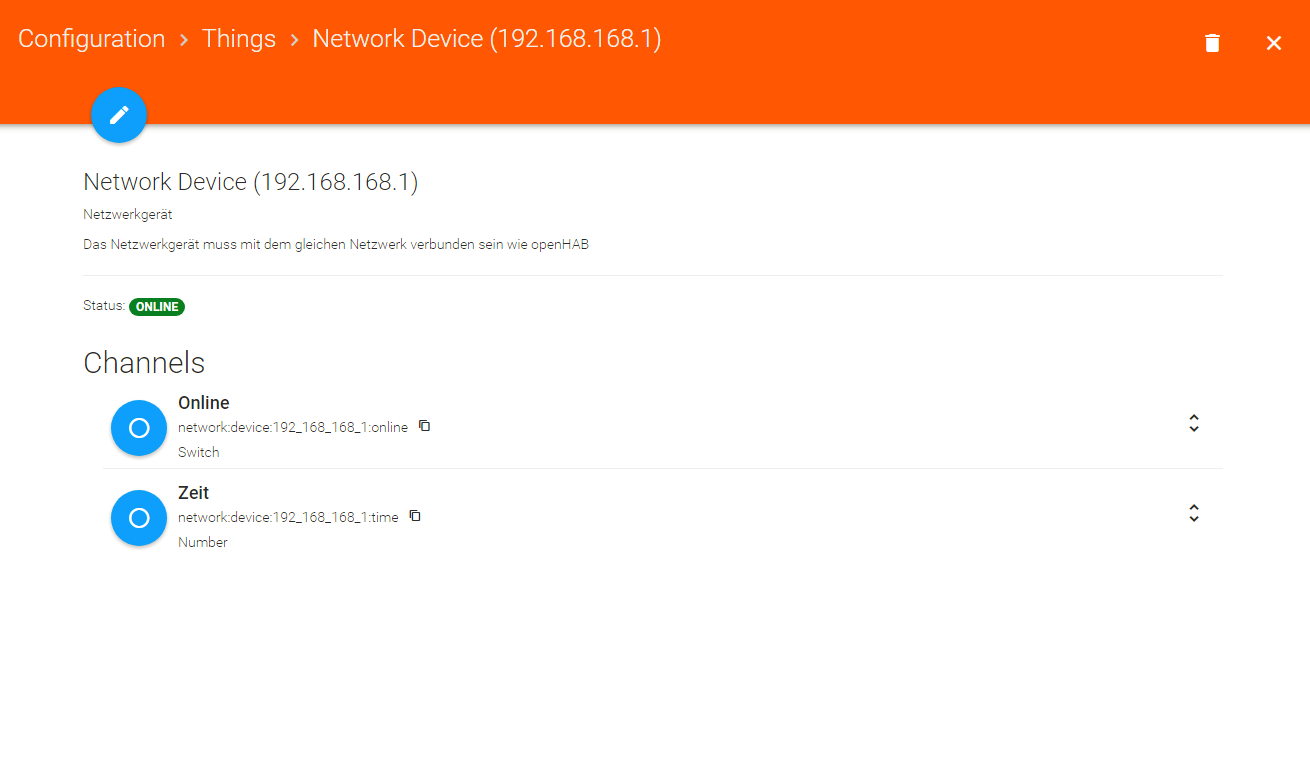
\includegraphics[width=0.9\textwidth]{Bilder/WLANthing.PNG}
	\caption{Menü des Gerätes}
	\label{fig:WLANthing}
\end{figure}

Hier kann bei Bedarf der Name geändert werden. Außerdem sieht man die verfügbaren Channels. Diese können einen bestimmten Wert einnehmen und mit einem Item verknüpft werden. Relevant ist in diesem Fall der Channel "'Online"', welcher anzeigt, ob das Gerät gerade mit dem Netzwerk verbunden ist. Mit einem Klick auf den Kreis erscheint ein Fenstermit einem Drop-Down-Menü, in dem alle verfügbaren Items aufgelistet sind, mit denen man den Channel verlinken kann. Außerdem kann ein neues Item erstellt werden, was in diesem Fall auch das Mittel der Wahl ist. 

\begin{figure}[H]
	\centering
	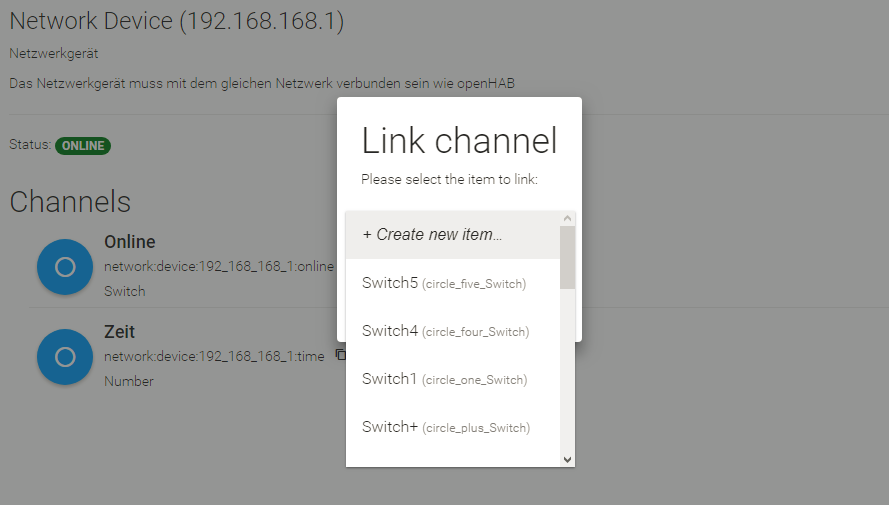
\includegraphics[width=0.9\textwidth]{Bilder/WLANchannel.PNG}
	\caption{Menü des Channels}
	\label{fig:WLANchannel}
\end{figure}

Damit gelangt man zum in \autoref{fig:linkChannel} gezeigten Menü. Hier kann man den Namen des Items ändern, diesen sollte man auch möglichst gut zuordnen können (z.B. Smartphone\_Status). Die weiteren Optionen werden so belassen.

\begin{figure}[H]
	\centering
	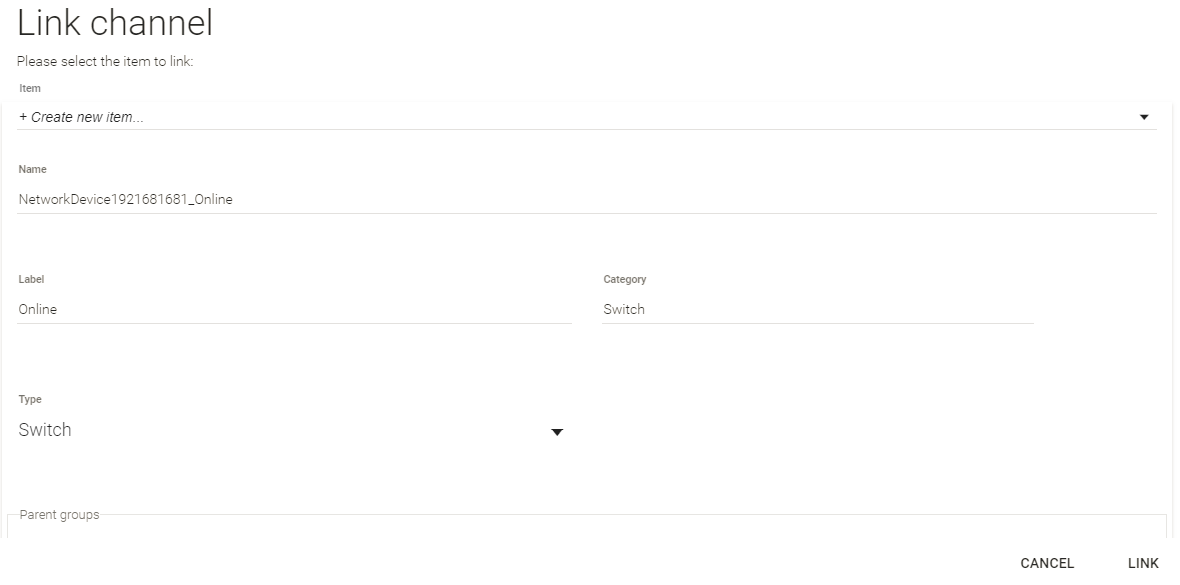
\includegraphics[width=0.9\textwidth]{Bilder/linkChannel.PNG}
	\caption{Link-Menü}
	\label{fig:linkChannel}
\end{figure}

Weiterhin muss das Item in anwesenheits.items eingefügt werden. Dies kann beispielsweise so aussehen:

\begin{lstlisting}
Switch smartphone "Smartphone" <light>
\end{lstlisting}

Für die Darstellung kann wie gewohnt ein Eintrag in smarthome.sitemap erstellt werden:
\begin{lstlisting}
Text item=smartphone label="Smartphone [MAP(praesenz.map):%s]" 
\end{lstlisting}

Auch hier wird das Mapping von "'ON"' zu "'Anwesend"' bzw. "'OFF"' zu "'Abwesend"' genutzt.

\paragraph{Gruppierung}
Damit die Benutzeroberfläche nicht zu unübersichtlich wird, wenn man mehrere Geräte/Methoden zur Anwesenheitserkennung nutzt, können die Geräte untereinander zu Gruppen zusammengefasst werden.

Binding: Network
Thing : IP-Adresse des Geräts
mit Item verbinden
Rules: Statusänderung
Gruppierung mit Gruppen

\subsection{RFID-Modul}

\subsubsection{Verbinden mit dem Raspberry Pi}

\begin{figure}[H]
	\centering
	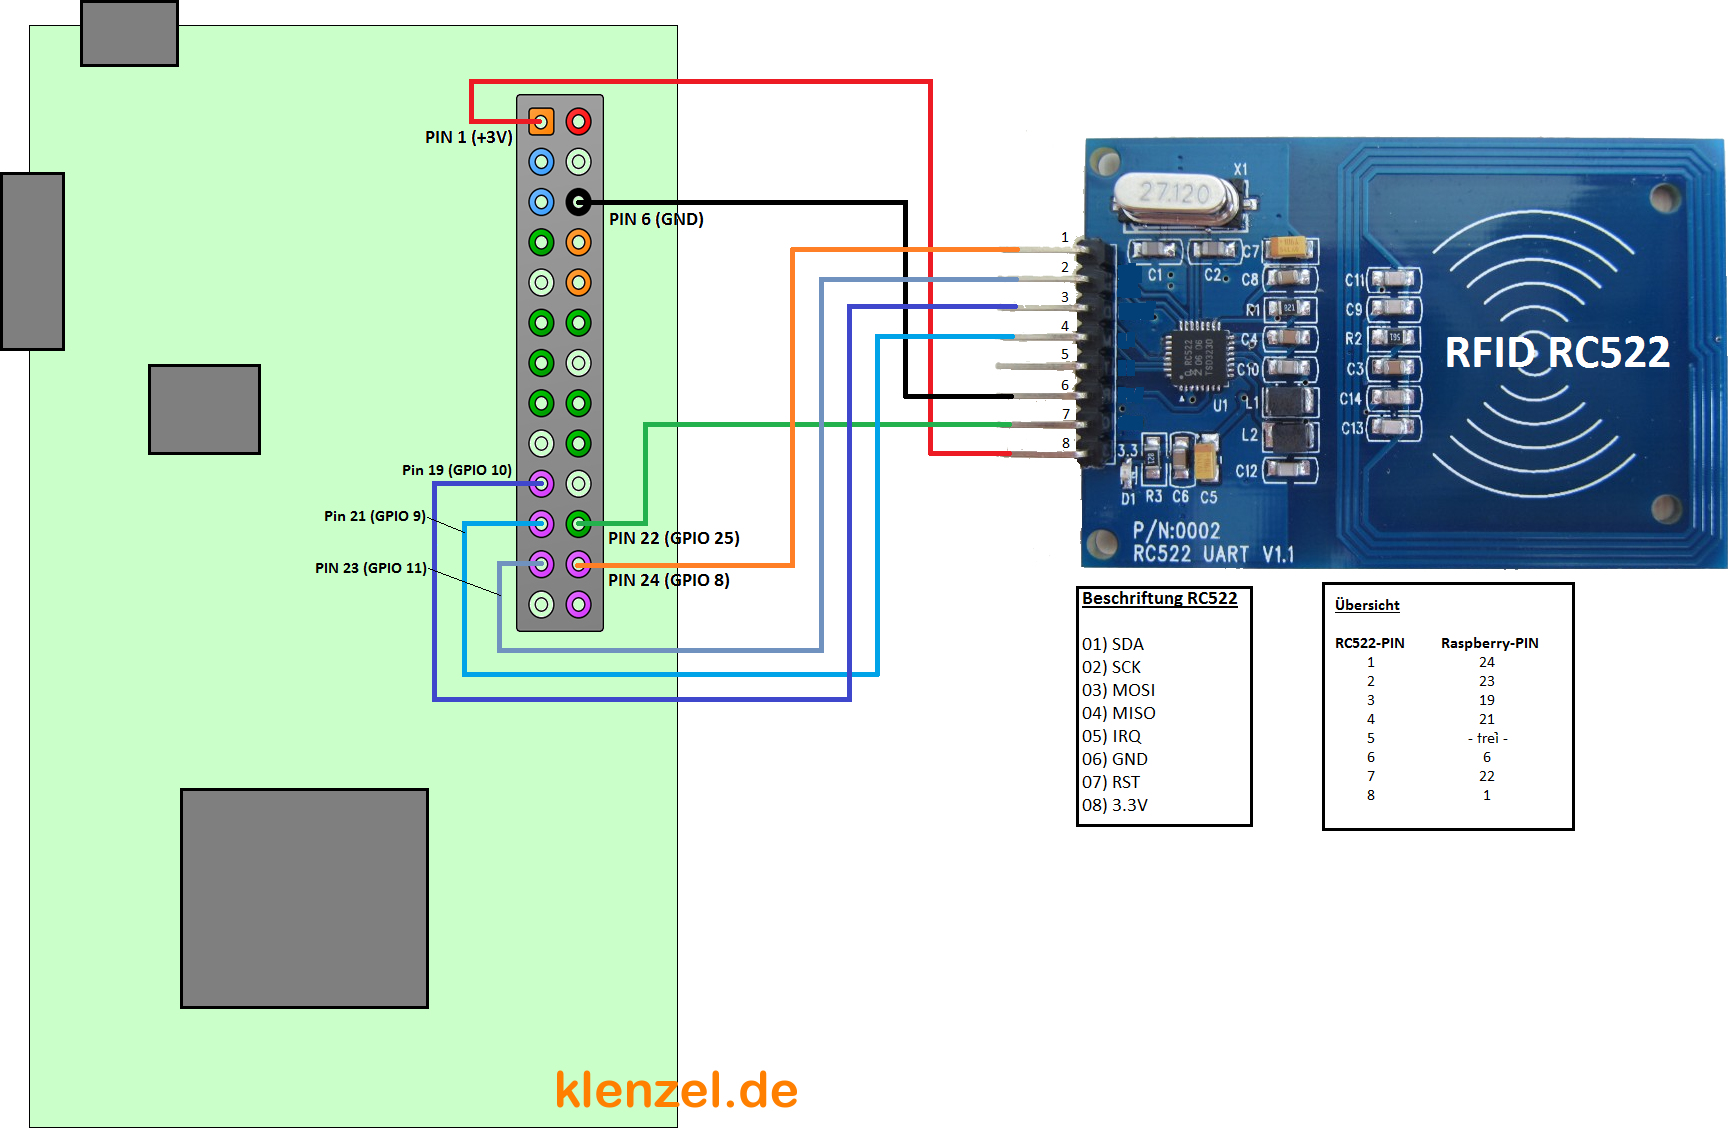
\includegraphics[width=0.9\textwidth]{Bilder/RFID.png}
	\caption{Verbinden des RFID-Moduls mit dem Raspberry Pi }
	\label{fig:RFID}
\end{figure}

Setup: https://tutorials-raspberrypi.de/raspberry-pi-rfid-rc522-tueroeffner-nfc/

\subsubsection{Python Skript}

\paragraph{State Machine}

\lstinputlisting[label=lst:stateMachine, caption = {Python-Skript mit State Machine zur Präsenzerkennung mit RFID-Modul}, language=Python]{lst/stateMachine.py}

